
\documentclass{article}
%encoding
%--------------------------------------
\usepackage[utf8]{inputenc}
\usepackage[T1]{fontenc}
%--------------------------------------
 
%German-specific commands
%--------------------------------------
\usepackage[ngerman]{babel}
\usepackage{csquotes}
%--------------------------------------

%Margins
%--------------------------------------
\usepackage{geometry}
 \geometry{
 a4paper,
 total={170mm,257mm},
 left=20mm,
 top=20mm,
 }
 
%Pictures
%--------------------------------------
\usepackage{graphicx}
\graphicspath{ {./Pictures/} }
\usepackage{tikz}
\usepackage{subcaption}
\usepackage{float}
\usepackage{wrapfig}
%--------------------------------------

%math
%--------------------------------------
\usepackage{amsmath}
\usepackage{amssymb}
\usepackage{amsfonts}
%--------------------------------------

%Frames
%--------------------------------------
\usepackage{framed}

%Own math commands
%--------------------------------------
\newcommand{\abs}[1]{\lvert#1\rvert}

%Colors
%--------------------------------------
\usepackage{xcolor}
\definecolor{blue-violet}{rgb}{0.54, 0.17, 0.89}
\definecolor{codegreen}{rgb}{0,0.6,0}
\definecolor{codegray}{rgb}{0.5,0.5,0.5}
\definecolor{codepurple}{rgb}{0.58,0,0.82}
\definecolor{backcolour}{rgb}{0.95,0.95,0.92}

%--------------------------------------
%\usepackage{multicol}
\usepackage{paracol}
\usepackage[shortlabels]{enumitem}

%Aufgaben
%--------------------------------------
\usepackage{amsthm}
\newtheorem{aufgabe}{Aufgabe}[section]
\newtheorem{definition}{Definition}[section]
\newtheorem{beispiel}{Beispiel}[section]
%--------------------------------------

%Listings
%--------------------------------------
\usepackage{ulem}
\usepackage{listings}
 
\lstdefinestyle{mystyle}{
    backgroundcolor=\color{backcolour},   
    commentstyle=\color{codegreen},
    keywordstyle=\color{magenta},
    numberstyle=\tiny\color{codegray},
    stringstyle=\color{codepurple},
    basicstyle=\ttfamily\footnotesize,
    breakatwhitespace=false,         
    breaklines=true,                 
    captionpos=b,                    
    keepspaces=true,                 
    numbers=left,                    
    numbersep=5pt,                  
    showspaces=false,                
    showstringspaces=false,
    showtabs=false,                  
    tabsize=2,
}
 
\lstset{style=mystyle,moredelim=[is][\sout]{|}{|}}
%--------------------------------------



\title{Funktionen in Tiger Jython}
\author{Alexandra Maximova}
\date{3. November 2020}

\begin{document}

\maketitle


\section{Aus kleinen Bausteinen grössere bauen} \label{section-ohne-parameter}

In Tiger Jython haben wir schon viele Befehle gesehen. Mit \lstinline|forward(100)|, zum Beispiel, bewegen wir die Schildkröte um 100 Schritte nach vorne, mit \lstinline|dot(25)| zeichnen wir einen Punkt vom Diameter 25. Bei anderen Wörter, wie zum Beispiel \lstinline|square(100)| oder \lstinline|circle(20)|, kriegen wir die Fehlermeldung, dass sie \emph{undefiniert} sind. Heisst das, dass wir sie selber \emph{definieren} können?

Ja! In Tiger Jython können wir Codestücke benennen und im Programm immer wieder verwenden. Das nennen wir eine \textbf{Funktion}. Im folgendem Codeabschnitt definieren wir eine Funktion \lstinline|quadrat100()|, die ein Quadrat mit Seitenlänge 100 zeichnet, und \textbf{rufen} diese zwei Mal \textbf{auf}.

\begin{figure}[H]
\centering
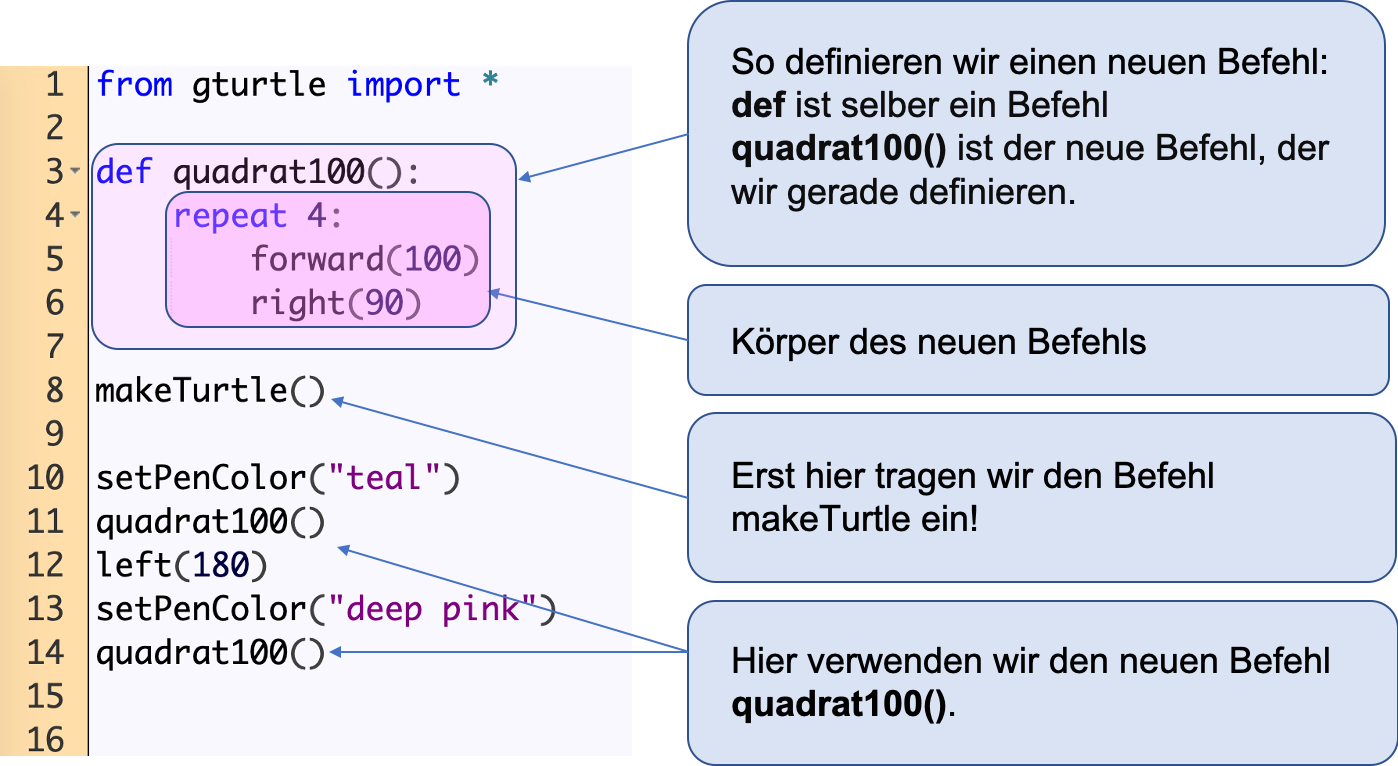
\includegraphics[width=0.6\linewidth]{pictures/definition_of_new_functions.png}
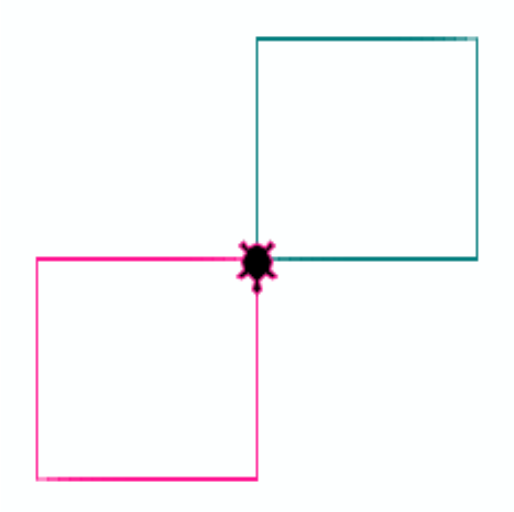
\includegraphics[width=0.3\linewidth]{pictures/def_example_picture.png}
\caption{Definition und Aufruf der Funktion \lstinline|quadrat100()|.} 
\end{figure}

Achtung: Eine Funktion wird erst dann ausgeführt, wenn sie aufgerufen wird.

\begin{aufgabe}\label{aufgabe-fenster}
Definiere eine Funktion \lstinline|square()|, welche ein Quadrat zeichnet, und verwende sie, um folgendes Bild zu zeichnen.
\begin{figure}[H]
\centering

\includegraphics[width=0.15\linewidth]{pictures/picture-fenster.png}
\end{figure}
\end{aufgabe}

\begin{aufgabe} \label{aufgabe-sechseck}
Definiere eine Funktion \lstinline|triangle()|, welche ein gleichseitiges Dreieck zeichnet, und verwende sie, um folgendes Bild zu zeichnen.
\begin{figure}[H]
\centering
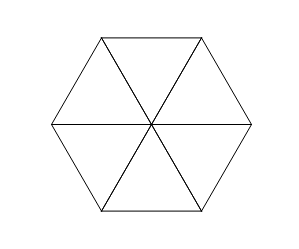
\includegraphics[width=0.2\linewidth]{pictures/picture-sechseck.png}
\end{figure}
\end{aufgabe}

\begin{aufgabe} \label{aufgabe-haus}
Fred und Gregory haben zwei Programme geschrieben, die das gleiche Bild zeichnen.

Kannst du erraten, was gezeichnet wird, ohne das Programm auszuführen? Bei welchem Programm findest du es einfacher?
\begin{paracol}{2}
\begin{figure}[H]
\lstinputlisting[language=Python, caption='Freds Programm']{programs/aufgabe-haus-fred.py}
\end{figure}

\switchcolumn

\begin{figure}[H]
\lstinputlisting[lastline=76,language=Python]{programs/aufgabe-haus-gregory.py}
\end{figure}
\begin{figure}[H]
\lstinputlisting[firstnumber=77,firstline=77,language=Python, caption='Gregorys Programm']{programs/aufgabe-haus-gregory.py}
\end{figure}

\end{paracol}

Ändere eins der Programme so, dass die Fenster keine einfachen Quadrate sind, sondern wie in Aufgabe \ref{aufgabe-fenster} aussehen.
\end{aufgabe}

\begin{aufgabe} \label{aufgabe-schokolade}
Zeichne diese Schokoladentafel. Überlege, welche Funktionen du definieren möchtest.
\begin{figure}[H]
\centering
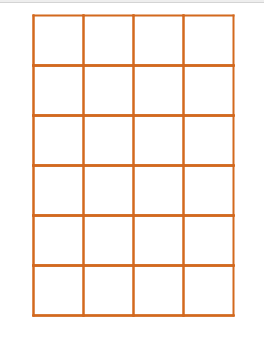
\includegraphics[width=0.2\linewidth]{pictures/picture-schokolade.png}
\end{figure}
\end{aufgabe}


\section{Befehle parametrisieren} \label{section-mit-parameter}

Bei den Befehlen \lstinline|forward(.)| und \lstinline|dot(.)| können wir angeben, um wie viel Schritte die Schildkröte nach vorne gehen soll oder wie gross der Punkt sein soll. Unsere selbstdefinierte Funktionen können das auch.

Zum Beispiel, müssen wir nicht für jede Dreiecksgrösse N eine eigene Funktion \lstinline|dreieckN()| definieren. Wir können die Funktion so definieren, dass sie einen Parameter \lstinline|seite| erwartet, welches die Länge einer Seite angibt.

\begin{figure}[H]
\centering
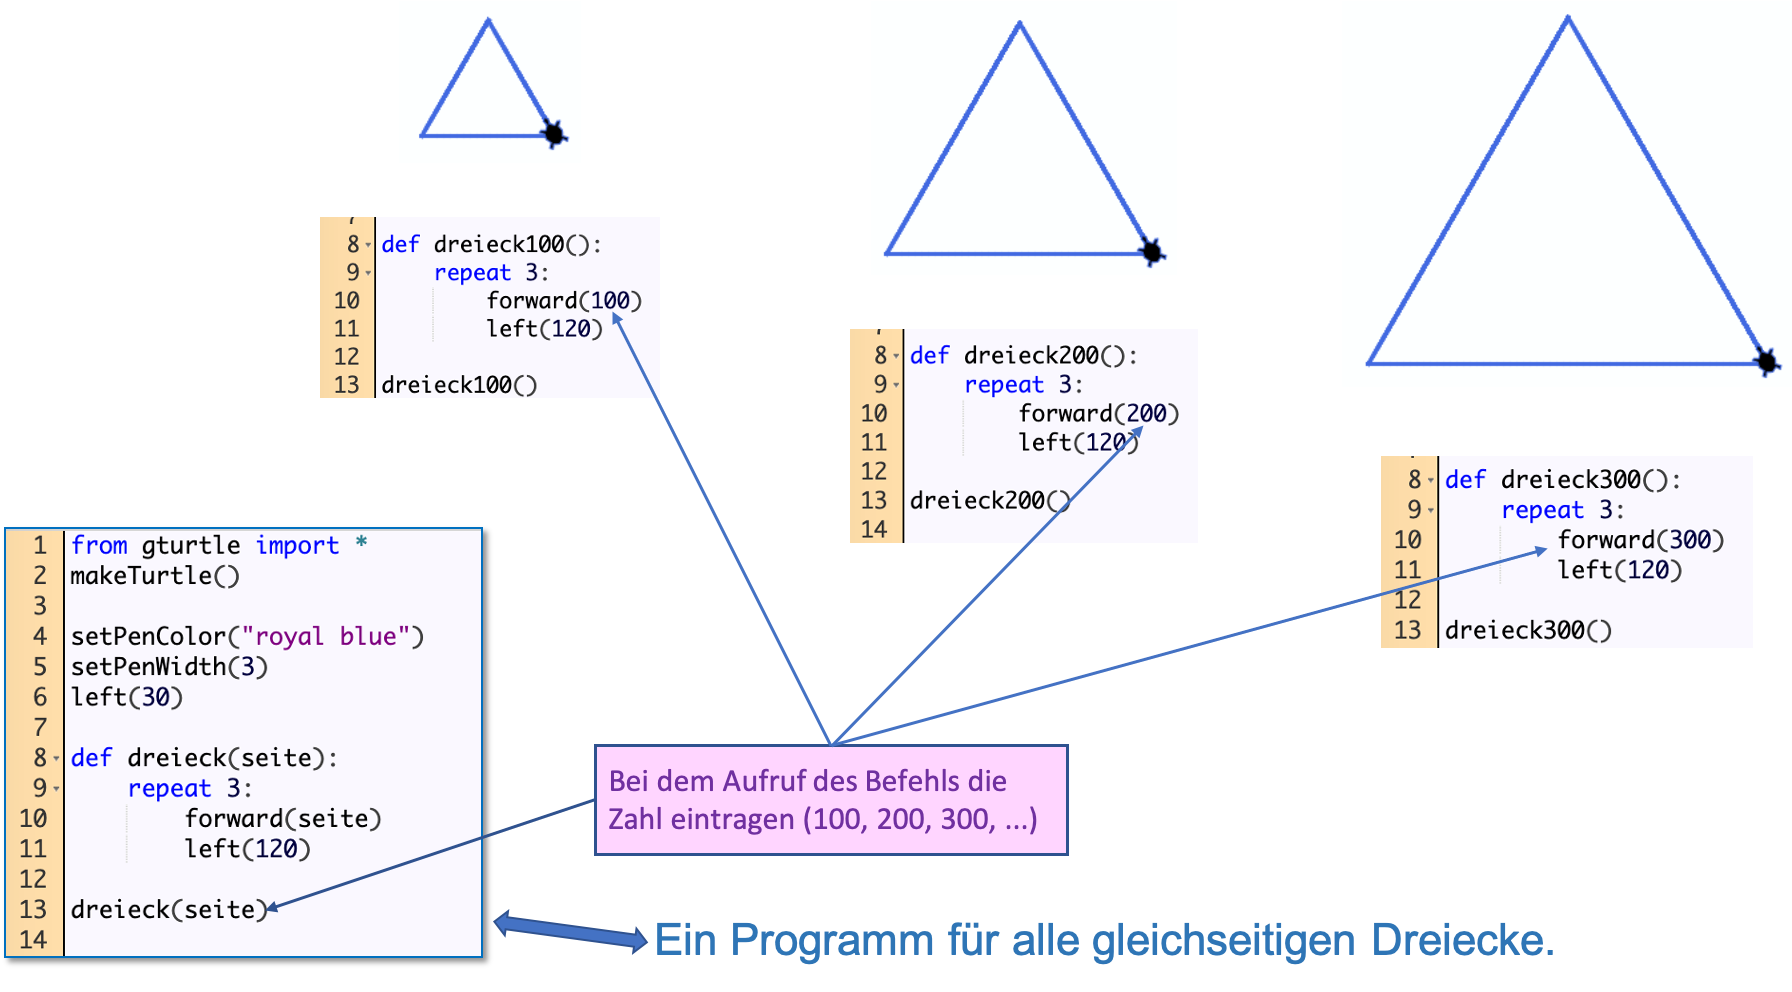
\includegraphics[width=0.8\linewidth]{pictures/overview_parameters_5.png} 
\end{figure}

\begin{aufgabe} \label{aufgabe-halbe-quadrate}
Definiere die Funktion \lstinline|square(side)|. Verwende sie, um folgendes Bild zu zeichnen.
\begin{figure}[H]
\centering
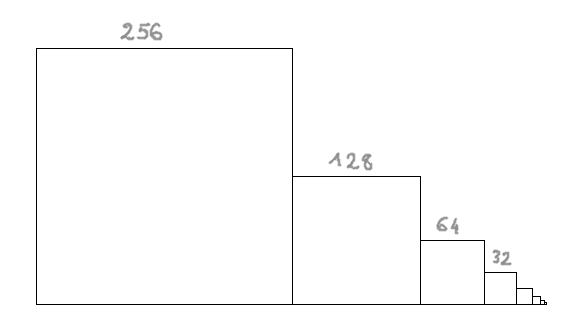
\includegraphics[width=0.35\linewidth]{pictures/picture-halbe-quadrate.png}
\end{figure}
\end{aufgabe}

\begin{aufgabe} \label{aufgabe-spiegel-korridor}
Zeichne folgendes Bild.
\begin{figure}[H]
\centering

\includegraphics[width=0.2\linewidth]{pictures/picture-spiegel-korridor.png}
\end{figure}
\end{aufgabe}

\begin{aufgabe} \label{aufgabe-roboter-gesicht}
Zeichne folgendes Robotergesicht aus Quadrate.
\begin{figure}[H]
\centering
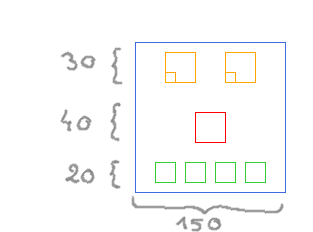
\includegraphics[width=0.25\linewidth]{pictures/picture-roboter-gesicht.png}
\end{figure}
\end{aufgabe}

\begin{aufgabe} \label{aufgabe-halbe-dreiecke}
Zeichne folgendes Bild. Die Seiten der Dreiecke halbieren sich jedes Mal. Überlege, welche Funktionen möchtest du definieren.
\begin{figure}[H]
\centering
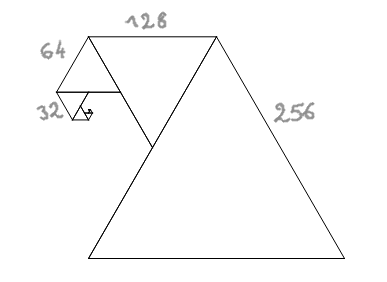
\includegraphics[width=0.3\linewidth]{pictures/picture-halbe-dreiecke.png}
\end{figure}
\end{aufgabe}

\begin{aufgabe} \label{aufgabe-polygone}
Zeichne folgendes Bild. Wie viele Funktionen musst du definieren? Reicht es, nur eine zu definieren?
\begin{figure}[H]
\centering

\includegraphics[width=0.35\linewidth]{pictures/picture-polygone.png}
\end{figure}
\end{aufgabe}

\newpage

\section*{Beispiellösungen}

\subsection*{Lösungen zu Abschnitt \ref{section-ohne-parameter}}

\paragraph{Aufgabe \ref{aufgabe-fenster}}
Dieses Programm definiert die Funktion \lstinline|square()| und zeichnet ein Fenster.
\lstinputlisting[language=Python]{programs/solution-fenster.py}

\paragraph{Aufgabe \ref{aufgabe-sechseck}} 
Dieses Programm definiert die Funktion \lstinline|triangle()| und zeichnet ein Sechseck.
\lstinputlisting[language=Python]{programs/solution-sechseck.py}

\paragraph{Aufgabe \ref{aufgabe-haus}} 
Beide Programme zeichnen ein Haus.
\begin{figure}[H]
\centering
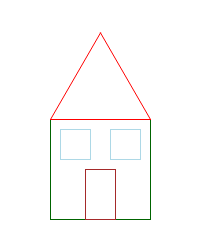
\includegraphics[width=0.3\linewidth]{pictures/picture-haus.png}
\end{figure}
Gregorys Programm zu verstehen und zu verändern sollte einfacher sein, weil sein Programm strukturierter ist und Funktionen verwendet. Insbesondere, es reicht, die Funktion \lstinline|window()| zu ändern, um andere Fenster zu zeichnen.

\lstinputlisting[language=Python,firstnumber=21,firstline=21,lastline=27]{programs/solution-haus-gregory.py}

\paragraph{Aufgabe \ref{aufgabe-schokolade}} 
Dieses Programm definiert die Funktion \lstinline|square()|, die Funktion \lstinline|row()| und zeichnet eine Tafel Schokolade.
\lstinputlisting[language=Python]{programs/solution-schokolade.py}

\subsection*{Lösungen zu Abschnitt \ref{section-mit-parameter}}

\paragraph{Aufgabe \ref{aufgabe-halbe-quadrate}}
Dieses Programm definiert die Funktion \lstinline|square(side)| und zeichnet immer kleiner werdende Quadrate.
\lstinputlisting[language=Python]{programs/solution-halbe-quadrate.py}

\paragraph{Aufgabe \ref{aufgabe-spiegel-korridor}}
Dieses Programm definiert die Funktion \lstinline|square(side)| und zeichnet verschachtelte immer kleiner werdende Quadrate.
\lstinputlisting[language=Python]{programs/solution-spiegel-korridor.py}

\paragraph{Aufgabe \ref{aufgabe-roboter-gesicht}} 
Dieses Programm definiert die Funktionen \lstinline|square(side)|, die ein Quadrat zeichnet, \lstinline|eye()|, \lstinline|nose()| und \lstinline|mouth()|, die jeweils Auge, Nase und Mund definieren und \lstinline|drawEyes()|, \lstinline|drawNose()| und \lstinline|drawMouth()|, welche jeweils Augen, Nase und Mund zentriert im Gesicht zeichen und wieder ans linke Gesichtsrand zurückkehren.
Diese Funktionen ermöglichen es uns, das eigentliche Zeichnen einfach und strukturiert zu halten.
\lstinputlisting[language=Python]{programs/solution-roboter-gesicht.py}

\paragraph{Aufgabe \ref{aufgabe-halbe-dreiecke}}
Dieses Programm definiert die Funktion \lstinline|triangle(side)| und zeichnet immer kleiner werdende Dreiecke.
\lstinputlisting[language=Python]{programs/solution-halbe-dreiecke.py}

\paragraph{Aufgabe \ref{aufgabe-polygone}}
Dieses Programm definiert die Funktion \lstinline|polygon(n)|, welches ein beliebiges n-Eck zeichen kann, und verwendet sie, um Drei- bis Siebenecken zu zeichnen.
\lstinputlisting[language=Python]{programs/solution-polygone.py}

\end{document}